\chapter{Results}

This chapter presents the progress and findings from the first phase of the project implementation. It includes project status reporting, initial testing outcomes demonstrating iterative architecture generation, quantitative evaluation utilizing natural language processing metrics, and a critical discussion of observed results.

\section{Project Implementation Status}

Development follows a two-phase schedule. The Phase 1 AWS-scoped prototype has largely been implemented, with the iterative feedback workflow successfully integrated with vector database. Key task progress is tracked and summarized in Table \ref{tab:project_status}, illustrating milestones completed and ongoing work.

\begin{table}[h]
    \centering
    \caption{Project Status}
    \label{tab:project_status}
    \begin{tabular}{@{}lll@{}}
        \toprule
        \textbf{Month} & \textbf{Planned Task} & \textbf{Status} \\
        \midrule
        August 2025 & Ideation & Completed \\
        September 2025 & Literature Review & Completed \\
         & Requirements Gathering & Completed \\
         & System Architecture Design & Completed \\
         & AWS Documentation Collection & Completed \\
        October 2025 & Vector Database Construction & Completed \\
         & Agentic Framework Development & Completed \\
        November 2025 & Evaluator--Optimizer Workflow Implementation & Completed \\
         & Testing \& Evaluation & In Progress \\
        \bottomrule
    \end{tabular}
\end{table}

\section{Preliminary Testing and Iterative Trace}

Initial qualitative testing validated the agentic evaluation-optimization graph logic. The system demonstrates the ability to iteratively refine solutions through multi-agent collaboration and validation feedback.

Below example with condensed format illustrates the system’s capability to recognize gaps and iteratively improve architectural proposals.

\begin{verbatim}
Input Query: "Guidance for Building a Containerized and Scalable Web Application on AWS" 

--- Iteration 1 --- 
Supervisor: Decomposing user problem into 4 domains: Compute, Network, Storage, Database. 
Generator Agents: Recommend solution:
    Compute: ECS on Fargate,
    Database: Aurora w/ RDS Proxy, 
    Network: VPC/ALB/CloudFront, 
    Storage: S3/EFS. 
Architect Synthesizer Agent:
    Proposed architecture: Build and integrate the components as...
Validaion Supervisor: Delegating validation tasks to domain validators.
Validator Agents: Feedback: 
    Compute: missing details (read-only FS, non-root). 
    Database: missing specifics (ElastiCache Multi-AZ, Proxy timeouts). 
    Network: valid.
    Storage: valid.
Validation Synthesizer:
    Validation Success: Partial (Minor revisions needed). 

--- Iteration 2 --- 

Supervisor: Re-evaluating. Integrating all components and addressing feedback. 
Generator Agents: Propose unified, 
    Compute: multi-account architecture integrating ECS
    Datbase: Multi AZ Aurora with ElasticCache
    Network: CloudFront+WAF 
    Storage: S3
Architect Synthesizer Agent:
    Proposed architecture: Build and integrate the components as...
Validaion Supervisor: Delegating validation tasks to domain validators.
Validator Agents: Feedback: 
    Compute: valid.
    Database: valid.
    Network: valid.
    Storage: valid.
Validation Synthesizer:
    Validation Success: Yes 
    
--- Final Output --- 
(Final architecture document generated: "Executive Summary - Objective: Deliver a secure, highly available, and scalable containerized web application platform on AWS...")
\end{verbatim}

\section{Quantitative Evaluation Strategy}

Architectural recommendations generated by the AI system are quantitatively evaluated against human expert-authored gold-standard references using three key NLP similarity metrics. 

\textbf{Note on Preliminary Status:} It is important to note that the quantitative results presented in this section are \textit{preliminary}. Due to the time constraints of Phase 1, a comprehensive evaluation across a large-scale dataset was not feasible. The data below represents an initial testing snapshot intended to validate the functional pipeline rather than final performance. A more rigorous evaluation is scheduled for Phase 2.

\subsection{ROUGE-L}

ROUGE-L measures recall-oriented longest common subsequence overlap between generated and reference texts, assessing lexical similarity \cite{lin2004rouge}.

\subsection{METEOR}

METEOR augments lexical alignment by incorporating stemming and synonymy, better capturing semantic equivalences \cite{banerjee2005meteor}.

\subsection{BERTScore}

BERTScore computes cosine similarity between contextual BERT embeddings of candidate and reference texts, providing robust semantic similarity assessment \cite{zhang2019bertscore}.

\section{Evaluation Metrics Report}

Table \ref{tab:evaluation-metrics} summarizes the precision, recall, and F1 scores computed against AWS references during this preliminary testing phase.

\begin{table}[h]
\centering
\caption{Evaluation Metrics Comparison Across System Phases}
\label{tab:evaluation-metrics}
\begin{tabular}{lccccccc}
\toprule
Phase           & ROUGE-L F1 & METEOR & BERTScore F1 \\
\midrule
Baseline (Plain LLM) & 0.117 & 0.180 & 0.572 \\
Agentic Draft        & 0.064 & 0.216 & 0.434 \\
Final System         & 0.066 & 0.209 & 0.438 \\
\bottomrule
\end{tabular}
\end{table}

\begin{figure}[H]
  \centering
  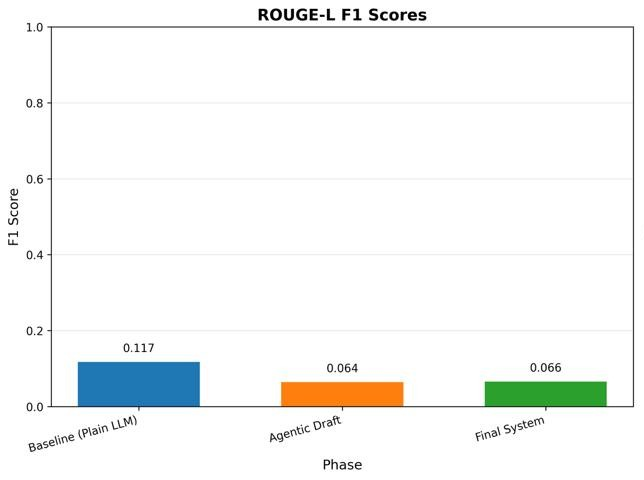
\includegraphics[width=10cm, height=8cm]{ROUGE-L.jpg}
  \caption{ROUGE-L Metric}
  \label{fig:ROUGE-L}
\end{figure}

\begin{figure}[H]
  \centering
  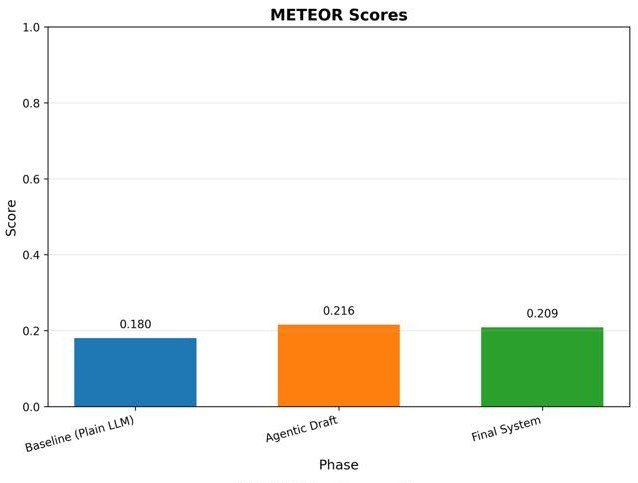
\includegraphics[width=10cm, height=8cm]{METEOR.jpg}
  \caption{METEOR Metric}
  \label{fig:METEOR}
\end{figure}

\begin{figure}[H]
  \centering
  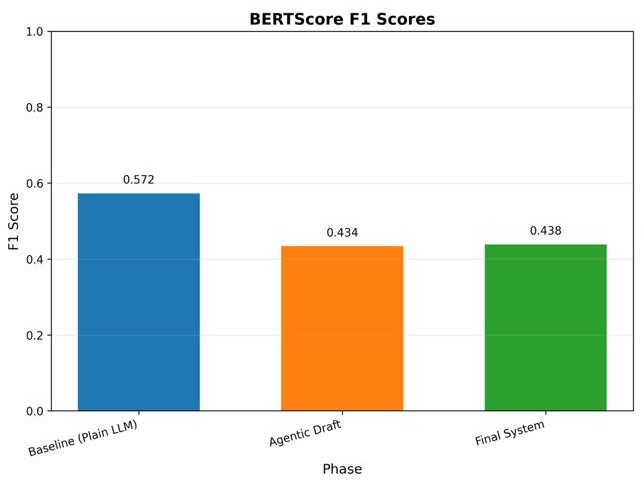
\includegraphics[width=10cm, height=8cm]{BERTScore.jpg}
  \caption{BERTScore Metric}
  \label{fig:BERTScore}
\end{figure}

\begin{figure}[H]
  \centering
  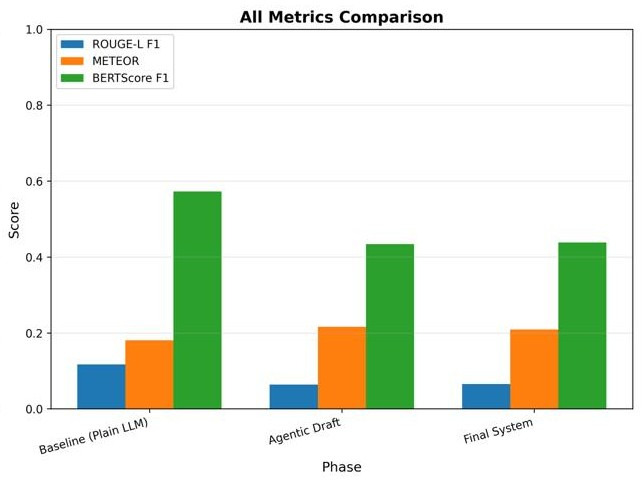
\includegraphics[width=10cm, height=8cm]{AllMetrics.jpg}
  \caption{All Metrics}
  \label{fig:All_Metrics}
\end{figure}


\section{Improvement Analysis}

Although the testing pool was limited due to time constraints, the preliminary metrics reveal distinct behavioral differences between the baseline (Zero-shot LLM) and the proposed Agentic Framework with and without feedback loop:

\begin{itemize}
    \item \textbf{Lexical Divergence (ROUGE-L):} The Baseline model achieved a higher ROUGE-L score ($0.117$) compared to the Agentic Draft ($0.064$). This indicates that the unprompted LLM mimics the general phrasing of the reference text (a "parroting" effect). However, the drop in ROUGE-L for the Agentic system is likely attributed to the RAG mechanism. The Agent retrieves specific technical excerpts from AWS documentation that may not exist in the high-level reference summary, leading to lower lexical overlap but arguably higher technical specificity.
    \item \textbf{Semantic Alignment (METEOR):} Crucially, the Agentic Draft outperformed the Baseline in the METEOR metric ($0.216$ vs $0.180$). Unlike ROUGE, METEOR accounts for synonyms and stemming. This improvement suggests that while the Agent uses different vocabulary (technical terms from documentation), it captures the \textit{conceptual essence} of the solution more accurately than the baseline.
    \item \textbf{Contextual Variance (BERTScore):} The decline in BERTScore ($0.572$ to $0.438$) highlights the "One-to-Many" challenge in cloud architecture. A single problem often has multiple valid solutions. The Agentic framework, influenced by retrieved documentation, often proposed valid modern alternatives (e.g., Fargate vs EC2) that differed structurally from the older "Gold Standard" references, resulting in a lower semantic similarity score despite potential technical validity.    
    A consolidated comparison of all metrics is presented in Figure \ref{fig:All_Metrics}.
\end{itemize}

\section{Interpretation and Discussion}

The Evaluator-Optimizer framework effectively enables iterative solution refinement. However, the preliminary results suggest a misalignment between standard NLP text-similarity metrics and the evaluation of complex architectural designs.

\begin{itemize}

    \item \textbf{Preliminary Nature of Data:} As noted, these results are derived from a limited testing window. However, they are sufficient to demonstrate the system's mechanical capability to iterate and modify solutions based on feedback.

    \item \textbf{The "Reference Trap":} Standard metrics assume one correct text sequence. The Agentic framework generated detailed, multi-component architectures that were penalized by metrics favoring brevity and generic phrasing.

    \item \textbf{Metric Misalignment:} The increase in METEOR scores coupled with the decrease in ROUGE indicates the system is optimizing for technical accuracy rather than linguistic mimicry. 

\end{itemize}

Therefore, while the current scores reflect the limitation of time and metric selection, they validate the underlying hypothesis: the agent is generating novel, grounded content rather than hallucinating generic text. A thorough evaluation incorporating functional correctness metrics is planned for the next phase.

\section{Summary}

Phase 1 validates the feasibility of agentic AI for cloud architecture recommendation, combining factual grounding with multi-agent iterative processing, setting the foundation for scalable multi-cloud support and enhanced evaluator optimization. Despite time constraints limiting the scope of testing, the system demonstrates successful iterative refinement and improved semantic alignment (METEOR). The preliminary data underscores the need for functional evaluation strategies in future work.
